\documentclass[conference]{IEEEtran}
\usepackage{cite}
\usepackage{amsmath,amssymb,amsfonts}
\usepackage{algorithmic}
\usepackage{graphicx}
\usepackage{textcomp}
\usepackage{xcolor}
\usepackage{booktabs}
\usepackage{hyperref}
\usepackage{pgfplots}
\pgfplotsset{compat=1.18}
\usepackage{fancyhdr}

\fancypagestyle{firstpage}{
  \fancyhf{}
  \renewcommand{\headrulewidth}{0pt}
  \fancyhead[C]{\small \textsf{Preprint. Available at \url{https://doi.org/10.5281/zenodo.18305656}}}
}

\def\BibTeX{{\rm B\kern-.05em{\sc i\kern-.025em b}\kern-.08em
    T\kern-.1667em\lower.7ex\hbox{E}\kern-.125emX}}

\begin{document}

\title{Deterministic Rematerialization: Convergent Evolution in Cloud Kernels and Edge Swarms}

\author{\IEEEauthorblockN{Cavin Krenik}
\IEEEauthorblockA{\textit{Department of Computer Science} \\
\textit{Olympic College}\\
Shelton, WA, USA \\
cavinkrenik@icloud.com}
}

\maketitle
\thispagestyle{firstpage}

\begin{abstract}
As AI scales in both parameter count (Large Language Models) and distribution (IoT Swarms), data movement---not arithmetic---has become the dominant cost. In the cloud, this appears as the ``logit bottleneck'': training stalls when massive intermediate tensors are written to and read from High Bandwidth Memory (HBM) during the final projection and cross-entropy loss. At the edge, it appears as the ``weight bottleneck'': federated nodes cannot afford to transmit dense model updates over constrained and unreliable RF links.

This paper identifies a structural isomorphism between two families of solutions that emerged independently: fused, IO-aware GPU kernels for cloud training (e.g., FlashAttention, Fused Cross-Entropy) and silent consensus for decentralized edge learning (QRES). We argue that both converge on the same strategy---\textbf{Deterministic Rematerialization}---in which intermediate state is intentionally discarded and later recomputed on demand, trading surplus compute for orders-of-magnitude reductions in IO. We further show that the two domains diverge on a key axis: cloud kernels frequently tolerate weak determinism due to parallel reductions, while edge swarms require strict determinism as a first-class constraint because ``silence'' is a correctness signal. We validate this thesis with a 10,000-node simulation demonstrating constant memory growth with respect to the number of peers, supporting the claim that determinism is not merely a constraint but an enabling technology for state-elision at scale.
\end{abstract}

\begin{IEEEkeywords}
Federated Learning, Edge AI, Systems Optimization, Determinism, IoT Swarms
\end{IEEEkeywords}

\section{Introduction}
Modern systems are increasingly limited by how much data they must move, not how many operations they can perform. This shift is visible at both extremes of the AI stack: datacenter GPUs constrained by memory bandwidth and edge swarms constrained by radio bandwidth. Although these environments differ radically in hardware and scale, they exhibit the same architectural outcome: they converge on recomputation to avoid movement.

\subsection{Two Gravity Wells}
\textbf{Datacenter gravity well (HBM bandwidth).} Training LLMs requires computing a cross-entropy loss over vocabularies that can exceed 128k tokens. The naive implementation materializes a $N \times V$ logit tensor (tokens $\times$ vocabulary), often requiring tens of gigabytes of memory just to produce a scalar loss \cite{narang2021efficient}. This creates a pathological pressure point at the final layer, triggering out-of-memory failures or forcing compromises such as aggressive micro-batching.

\textbf{Edge gravity well (RF spectrum).} Federated and swarm-learning systems must synchronize models across links such as LoRa, LTE-M, or intermittent WiFi. Dense model deltas can be megabytes to gigabytes at modern scales, making frequent transmission infeasible in bandwidth, latency, and energy. Any architecture that requires global state shipment as a steady-state behavior rapidly saturates the network and drains node batteries.

\subsection{Convergent Evolution: The Compute-for-IO Trade}
Under these constraints, both domains independently evolved the same pattern: IO avoidance via recomputation.

\begin{itemize}
    \item \textbf{Cloud Kernels:} IO-aware fused kernels reduce the logit bottleneck by avoiding the write-read cycle of intermediate tensors. Instead of materializing $N \times V$ logits in HBM, the kernel computes small tiles in registers, maintains running statistics (e.g., online softmax), emits only the scalar loss, and discards the tile immediately \cite{dao2022flashattention}.
    \item \textbf{Edge Swarms (QRES):} QRES is a deterministic, fixed-point federated learning runtime that replaces state transmission with silent consensus via replay. Rather than transmitting full updates, nodes transmit minimal residual information and rely on local simulation to reconstruct the neighbor's state.
\end{itemize}

The shared rule is simple: \textit{Intermediate tensors are optional if they can be rematerialized reproducibly.} Understanding this convergence matters because it suggests a unifying design principle for future AI systems: treat intermediate state as ephemeral, and design determinism as a first-class system property.

\subsection{The Determinism Gap}
The mechanism is shared, but the correctness requirements differ. Cloud kernels often accept \textbf{weak determinism}, depending on parallel reductions where floating-point associativity errors are tolerable. Edge swarms, however, require \textbf{strict determinism}. In the QRES architecture, silence is interpreted as agreement; even small numerical drift can fracture synchronization. Therefore, QRES treats bit-perfect reproducibility as the enabling condition that makes large-scale state elision safe.

\section{A Unified Model of Data Movement Minimization}
To formalize the convergence between cloud kernels and edge swarms, we abstract away the specific hardware and define a generalized cost model for learning systems constrained by data movement.

\subsection{The Cost of State}
We define the total cost $T$ of a learning step as a function of discrete messages, data volume, and computation:

\begin{equation}
    T = \alpha \cdot M + \beta \cdot B + \gamma \cdot F
\end{equation}

Where:
\begin{itemize}
    \item $M$ = number of messages or kernel launches
    \item $B$ = total bytes moved (over HBM or RF)
    \item $F$ = floating-point operations performed
\end{itemize}

In the ``bottleneck'' regimes we study, $\beta \gg \gamma$. This inequality shifts the optimal strategy toward recomputation: it becomes cheaper to perform redundant math ($\uparrow F$) than to persist and move state ($\downarrow B$).

\subsection{The Rematerialization Operator}
We coin this shared pattern \textbf{Deterministic Rematerialization} ($\mathcal{R}$), a tripartite operator that transforms a high-bandwidth process into a high-compute process:
\begin{enumerate}
    \item \textbf{Discard:} Do not write the full state tensor $S$ to the persistent medium.
    \item \textbf{Retain:} Persist only a minimal sufficient statistic $\phi(S)$ such that $|\phi(S)| \ll |S|$.
    \item \textbf{Replay:} When $S$ is required, reconstruct it exactly via a deterministic function $f$: $S' = f(\phi(S))$.
\end{enumerate}

For this operator to be valid, the reconstruction must be \textbf{semantically lossless} (statistically equivalent in cloud kernels; bitwise identical in edge swarms).

\subsection{Structural Isomorphism}
Table \ref{tab:iso} maps the implementation of this operator across the two domains.

\begin{table}[htbp]
\caption{Structural Isomorphism of Rematerialization}
\begin{center}
\begin{tabular}{@{}lll@{}}
\toprule
\textbf{Feature} & \textbf{Cloud (Fused Kernels)} & \textbf{Edge (QRES)} \\ \midrule
Constraint ($\beta$) & HBM Bandwidth & RF Spectrum \\
Heavy State ($S$) & Logits ($N \times V$) & Gradients ($W$) \\
Light Statistic ($\phi$) & Softmax Max/Sum & Consensus Residuals \\
Discard Mechanism & Tiling & Silence \\
Replay Mechanism & Recomputation & Local Simulation \\
Failure Mode & Numerical drift & Traffic storm \\ \bottomrule
\end{tabular}
\label{tab:iso}
\end{center}
\end{table}

\subsection{The Determinism Spectrum}
While the operator is universal, the tolerance for drift is not. \textbf{Weak determinism} is tolerable only when coordination is centralized and corrective feedback is cheap. \textbf{Strict determinism} is required when coordination is decentralized and feedback is expensive. In QRES, if Node A and Node B diverge by a single bit, the ``Silent Consensus'' assumption breaks. Thus, fixed-point arithmetic (Q16.16) is not an optimization but a topological necessity. We note that approximate rematerialization (e.g., stochastic or lossy replay) remains viable in centralized settings but becomes unstable under decentralized coordination.

\subsection{Empirical Validation: The Empty Bucket}
We validated the ``state elision'' hypothesis via a 10,000-node simulation on a single 2-vCPU Azure instance. Nodes were instantiated as time-multiplexed logical peers executing identical deterministic training steps within a fixed memory arena, isolating algorithmic state growth from allocator artifacts.

\begin{figure}[htbp]
\centering
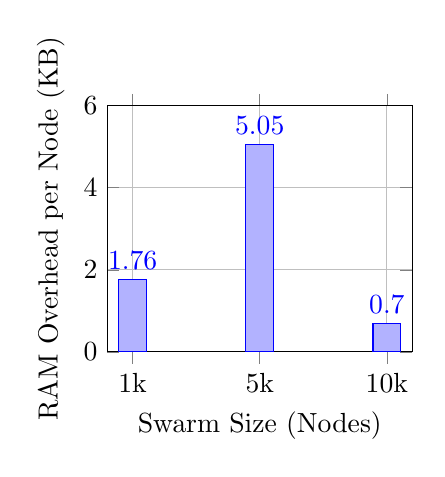
\begin{tikzpicture}
\begin{axis}[
    ybar,
    symbolic x coords={1k, 5k, 10k},
    xtick=data,
    ylabel={RAM Overhead per Node (KB)},
    xlabel={Swarm Size (Nodes)},
    ymin=0, ymax=6,
    nodes near coords,
    grid=major,
    width=0.45\textwidth
]
\addplot coordinates {(1k,1.76) (5k,5.05) (10k,0.70)};
\end{axis}
\end{tikzpicture}
\caption{The ``Empty Bucket'' Effect: As the swarm scales to 10k nodes, constant-size arenas are reused across epochs, driving marginal memory cost toward zero.}
\label{fig:memory}
\end{figure}

As shown in Fig. \ref{fig:memory}, the marginal memory cost drops significantly at scale. This confirms that the runtime is not persisting global state ($O(N)$), but rather re-materializing it ($O(1)$) into pre-allocated memory pages (``buckets'') that are reused across peer interactions.

\section{Case Studies}

\subsection{Cloud: Fused Linear--Cross-Entropy}
In LLM training, the final layer projects the hidden state $H$ into the vocabulary $V$ to produce logits $Y = HW$. Standard implementations materialize $Y$ in HBM, consuming $O(Batch \times Vocab)$. Optimizations such as fused cross-entropy kernels \cite{narang2021efficient} and FlashAttention \cite{dao2022flashattention} apply Deterministic Rematerialization by computing tiles of $Y$ in SRAM, calculating only the running \texttt{max} and \texttt{sum}, and discarding the tile. During backward, the kernel re-computes the specific tile needed. This reduces memory complexity from $O(V)$ to $O(1)$ per thread block.

\subsection{Edge: QRES Silent Consensus}
In the QRES architecture, the ``Weight Bottleneck'' prevents transmission of updates $\Delta W$. Nodes share only the ``Surprise'' (a bounded residual error signal). Each node independently re-runs the training step on its local replica. Because the core math is bit-perfect Q16.16, the local replay yields a $\Delta W'$ identical to the sender's $\Delta W$. This reduces network complexity from $O(ModelSize)$ to $O(Residual)$.

\subsection{Comparative Failure Analysis}
The divergence in determinism requirements is driven by the asymmetry of failure costs.

\textbf{Cloud Failure (Accuracy Cost):} In cloud training, floating-point non-associativity causes minor gradient drift. While end-to-end pipelines may be non-deterministic, kernel-level rematerialization typically maintains statistical equivalence. Drift here is indistinguishable from SGD noise and does not impede convergence \cite{jain2019reproducibility}.

\textbf{Edge Failure (Bandwidth Cost):} In QRES, silence implies agreement. If Node A (ARM) and Node B (x86) diverge by a single bit ($\epsilon > 0$), the consensus hash fractures. Node B rejects the update as ``Byzantine,'' triggering a fallback synchronization.
\begin{itemize}
    \item \textit{Cost of Success:} 0 bytes (Silent).
    \item \textit{Cost of Failure:} $ModelSize \times Neighbors$.
\end{itemize}
For a 10MB model in a 50-neighbor swarm, a single non-deterministic bit triggers a \textbf{500MB traffic storm}. Thus, strict Q16.16 determinism is an economic necessity to avoid catastrophic bandwidth spikes.

\section{Related Work}

\subsection{IO-Aware Cloud Training}
The bottleneck of memory bandwidth in GPU training has driven a surge in ``IO-aware'' kernel design. Chen et al. \cite{chen2016training} introduced \textit{Gradient Checkpointing}, demonstrating that recomputing activations during the backward pass could reduce memory requirements from $O(N)$ to $O(\sqrt{N})$. Dao et al. \cite{dao2022flashattention} extended this to attention mechanisms, proving that tiling computations in SRAM to avoid HBM access yields significant wall-clock speedups. Our work generalizes these findings, applying the same ``recompute-over-persist'' principle to the network layer.

\subsection{Federated Learning \& Compression}
Traditional Federated Learning (FL) relies on model compression to mitigate bandwidth constraints. Techniques such as gradient quantization, sparsification, and top-$k$ selection reduce the size of the update payload $\Delta W$ \cite{kairouz2021advances}. However, these methods remain rooted in the paradigm of \textit{state transmission}. QRES diverges by shifting to \textit{state simulation}: instead of compressing the message, we elide it entirely.

\subsection{Determinism in Distributed Systems}
While reproducibility is a standard goal in ML ops, it is rarely treated as a correctness constraint \cite{jain2019reproducibility}. In contrast, distributed systems often rely on state machine replication for correctness \cite{geels2006frugal}. QRES bridges these worlds by applying the strict determinism of consensus algorithms to the stochastic process of neural training.

\section{Conclusion}
We are entering an era of \textbf{Implicit State}. Whether in a GPU cluster or a drone swarm, the most efficient way to share massive state is not to send it, but to recreate it. This paper demonstrated that ``Fused Kernels'' and ``Silent Consensus'' are manifestations of the same \textbf{Deterministic Rematerialization} operator. The QRES results (10,000 nodes, $O(1)$ memory) provide empirical proof that strict determinism is the key to breaking the linear relationship between network scale and resource consumption.

We expect deterministic rematerialization to become increasingly relevant as systems push toward on-device learning. This raises a new challenge for compiler design: \textbf{Can we build ``deterministic compilers'' that optimize not just for speed, but for bitwise reproducibility across heterogeneous ISAs?} Solving this would allow silent consensus to scale beyond homogeneous swarms to planetary-scale, multi-architecture grids without explicit synchronization.

\bibliographystyle{IEEEtran}
\bibliography{references}

\end{document}
